
\documentclass[11pt]{article}

%% PACKAGES
\usepackage{graphicx}
\usepackage{verbatim}
\usepackage{url}
\usepackage[printonlyused]{acronym}
\usepackage[ruled]{algorithm}
\usepackage{amsmath,amssymb,amsfonts,amsthm}
\usepackage{overpic}
\usepackage{calc}
\usepackage{color}
 \usepackage[margin=1.0in]{geometry}
\usepackage[colorlinks=false]{hyperref}
\usepackage{textcomp}
\usepackage{cite}
\usepackage{mdwlist}
\usepackage{subfiles}
\usepackage{enumitem}
\usepackage{calc}
\usepackage{array}
\usepackage{units}
\usepackage{arydshln,leftidx,mathtools}
\usepackage[caption=false,font=footnotesize]{subfig}
\usepackage{relsize}
\usepackage{float}
\usepackage{makecell}
\usepackage{xr}
\usepackage{tabularx}

\usepackage{algorithm}
\usepackage[noend]{algpseudocode}

\setcounter{secnumdepth}{3}

\makeatletter
\let\@tmp\@xfloat     
\usepackage{fixltx2e}
\let\@xfloat\@tmp                    
\makeatother

\usepackage[subfigure]{tocloft}
\usepackage[singlespacing]{setspace}

\usepackage{pgfplots}

\usepackage{cancel}

\usepackage{tikz}
\usetikzlibrary{calc,patterns,decorations.pathmorphing,decorations.markings,fit,backgrounds}

\usepackage[strict]{changepage} %use to manually place figs/tables to get them within the margins

\makeatletter
\g@addto@macro\normalsize{%
  \setlength\abovedisplayskip{0.25pt}
  \setlength\belowdisplayskip{0.25pt}
  \setlength\abovedisplayshortskip{0.25pt}
  \setlength\belowdisplayshortskip{0.25pt}
}
\makeatother



\setlength{\parskip}{\baselineskip}

%% GRAPHICS PATH
\graphicspath{{../../../shared_latex_inputs/images}{../../../shared_latex_inputs/graphs}}

%% TODO
\newcommand{\todo}[1]{\vspace{5 mm}\par \noindent \framebox{\begin{minipage}[c]{0.98 \columnwidth} \ttfamily\flushleft \textcolor{red}{#1}\end{minipage}}\vspace{5 mm}\par}

%% MACROS
\providecommand{\abs}[1]{\lvert#1\rvert}
\providecommand{\norm}[1]{\lVert#1\rVert}
\providecommand{\dualnorm}[1]{\norm{#1}_\ast}
\providecommand{\set}[1]{\lbrace\,#1\,\rbrace}
\providecommand{\cset}[2]{\lbrace\,{#1}\nobreak\mid\nobreak{#2}\,\rbrace}
\providecommand{\onevect}{\mathbf{1}}
\providecommand{\zerovect}{\mathbf{0}}
\providecommand{\field}[1]{\mathbb{#1}}
\providecommand{\C}{\field{C}}
\providecommand{\R}{\field{R}}
\providecommand{\polar}{\triangle}
\providecommand{\Cspace}{\mathcal{Q}}
\providecommand{\Fspace}{\mathcal{F}}
\providecommand{\free}{\text{\{}\mathsf{free}\text{\}}}
\providecommand{\iff}{\Leftrightarrow}
\providecommand{\qstart}{q_\text{initial}}
\providecommand{\qgoal}{q_\text{final}}
\providecommand{\contact}[1]{\Cspace_{#1}}
\providecommand{\feasible}[1]{\Fspace_{#1}}
\providecommand{\prob}[2]{p(#1|#2)}
\providecommand{\prior}[1]{p(#1)}
\providecommand{\Prob}[2]{P(#1|#2)}
\providecommand{\Prior}[1]{P(#1)}
\providecommand{\parenth}[1] {\left(#1\right)}
\providecommand{\braces}[1] {\left\{#1\right\}}
\providecommand{\micron}{\hbox{\textmu m}}

%% MATH FUNCTION NAMES
\DeclareMathOperator{\conv}{conv}
\DeclareMathOperator{\cone}{cone}
\DeclareMathOperator{\homog}{homog}
\DeclareMathOperator{\domain}{dom}
\DeclareMathOperator{\range}{range}
\DeclareMathOperator{\argmax}{arg\,max}
\DeclareMathOperator{\argmin}{arg\,min}
\DeclareMathOperator{\area}{area}
\DeclareMathOperator{\sign}{sign}
\DeclareMathOperator{\mathspan}{span}
\DeclareMathOperator{\sn}{sn}
\DeclareMathOperator{\cn}{cn}
\DeclareMathOperator{\dn}{dn}
\DeclareMathOperator*{\minimize}{minimize}

\DeclareMathOperator{\atan2}{atan2}

\newtheorem{theorem}{Theorem}
\newtheorem{lemma}[theorem]{Lemma}

\title{{\Huge EMTG Tutorial: Constraint Scripting}}
\vspace{0.5cm}
\author
{
	Tim Sullivan \thanks{Aerospace Engineer, The Aerospace Corporation}
}
\vspace{0.5cm}


\newcommand{\listofknownissuesname}{\Large List of Known Issues}
\newlistof{knownissues}{mcf}{\listofknownissuesname}

\newcommand{\knownissue}[3]
{
	\refstepcounter{knownissues}
	\par\noindent\textbf{\hyperref[#2_b]{\theknownissues\quad #1}}\label{#2_h}
	\textbf{\hfill\pageref{#2_b}}
	#3
}

\newcommand{\knownissuelabel}[2]
{
	 \phantomsection
  	\hyperref[#2_h]{#1}\def\@currentlabel{\unexpanded{#1}}\label{#2_b}
}

\begin{document}

\begin{titlepage}
\maketitle
\thispagestyle{empty}
\begin{table}[H]
	\centering
	\begin{tabularx}{\textwidth}{|l|l|X|}
		\hline
		\textbf{Revision Date} & \textbf{Author} & \textbf{Description of Change} \\
		\hline
		\date{December 2, 2022} & Tim Sullivan & Initial revision.\\
		\hline
		\date{August 4, 2023} & Joseph Hauerstein & Addition of Known Issues section.\\ 
		\hline
	\end{tabularx}
\end{table}
\end{titlepage}

\newpage
\listofknownissues
\thispagestyle{empty}

\knownissue{Final state in ephemeris file may not have the final burn included}{missing_capture_burn_issue}

\newpage
\clearpage
\setcounter{page}{1}



\section*{List of Acronyms}
\begin{acronym}
%To define the acronym and include it in the list of acronyms: \acro{acronym}{definition}
%To define the acronym and exclude it from the list of acronyms:  \acro{acronym}{definition}
%
%\ac{acronym} Expand and identify the acronym the first time; use only the acronym thereafter
%\acf{acronym} Use the full name of the acronym.
%\{acronym} Use the acronym, even before the first corresponding \ac command
%\acl{acronym}  Expand the acronym without using the acronym itself.
%
%

\acro{ACS}{attitude control system}
\acro{ACO}{Ant Colony Optimization}
\acro{AD}{Automatic Differentiation}
\acro{ADL}{Architecture Design Laboratory}
\acro{AES}{Advanced Exploration Systems}
\acro{AGA}{aerogravity assist}
\acro{ALARA}{As Low As Reasonably Achievable}
\acro{API}{application programming interface}
\acro{BB}{branch and bound}
\acro{BVP}{Boundary Value Problem}
\acro{CATO}{Computer Algorithm for Trajectory Optimization}
\acro{CL}{confidence level}
\acro{CONOPS}{concept of operations}
\acro{COV}{Calculus of Variations}
\acro{D/AV}{Descent/Ascent Vehicle}
\acro{DE}{Differential Evolution}
\acro{DLA}{Declination of Launch Asymptote}
\acro{RLA}{Right Ascension of Launch Asymptote}
\acro{RA}{right ascension}
\acro{DEC}{declination}
\acro{DPTRAJ/ODP}{Double Precision Trajectory and Orbit Determination Program}
\acro{DSH}{Deep Space Habitat}
\acro{DSN}{Deep Space Network}
\acro{DSMPGA}{Dynamic-Size Multiple Population Genetic Algorithm}
\acro{EB}{Evolutionary Branching}
\acro{ECLSS}{environmental control and life support system}
\acro{ELV}{expendable launch vehicle}
\acro{EMME}{Earth to Mars, Mars to Earth}
\acro{EMMVE}{Earth to Mars, Mars to Venus to Earth}
\acro{EMTG}{Evolutionary Mission Trajectory Generator}
\acro{EVMME}{Earth to Venus to Mars, Mars to Earth}
\acro{EVMMVE}{Earth to Venus to Mars, Mars to Venus to Earth}
\acro{ERRV}{Earth Return Re-entry Vehicle}
\acro{FISO}{Future In-Space Operations}
\acro{FMT}{Fast Mars Transfer}
\acro{GASP}{Gravity Assist Space Pruning}
\acro{GCR}{galactic cosmic radiation}
\acro{GRASP}{Greedy Randomized Adaptive Search Procedure}
\acro{GSFC}{Goddard Space Flight Center}
\acro{GTOC}{Global Trajectory Optimization Competition}
\acro{GTOP}{Global Trajectory Optimization Problem}
\acro{HAT}{Human Architecture Team}
\acro{HGGA}{Hidden Genes Genetic Algorithm}
\acro{IMLEO}{Initial Mass in \acl{LEO}}
\acro{IPOPT}{Interior Point OPTimizer}
\acro{ISS}{International Space Station}
\acro{JHUAPL}{Johns Hopkins University Applied Physics Laboratory}
\acro{JSC}{Johnson Space Center}
\acro{KKT}{Karush-Kuhn-Tucker}
\acro{LEO}{Low Earth Orbit}
\acro{LRTS}{lazy race tree search}
\acro{MONTE}{Mission analysis, Operations, and Navigation Toolkit Environment}
\acro{MCTS}{Monte Carlo tree search}
\acro{MGA}{Multiple Gravity Assist}
\acro{MIRAGE}{Multiple Interferometric Ranging Analysis using GPS Ensemble}
\acro{MOGA}{Multi-Objective Genetic Algorithm}
\acro{MOSES}{Multiple Orbit Satellite Encounter Software}
\acro{MPI}{message passing interface}
\acro{MPLM}{Multi-Purpose Logistics Module}
\acro{MSFC}{Marshall Space Flight Center}
\acro{NELLS}{NASA Exhaustive Lambert Lattice Search}
\acro{NSGA}{Non-Dominated Sorting Genetic Algorithm}
\acro{NSGA-II}{Non-Dominated Sorting Genetic Algorithm II}
\acro{NHATS}{Near-Earth Object Human Space Flight Accessible Targets Study}
\acro{NTP}{Nuclear Thermal Propulsion}
\acro{OD}{orbit determination}
\acro{OOS}{On-Orbit Staging}
\acro{PCC}{Pork Chop Contour}
\acro{PEL}{permissible exposure limits}
\acro{PLATO}{PLAnetary Trajectory Optimization}
\acro{REID}{risk of exposure-induced death}
\acro{RTBP}{Restricted Three Body Problem}
\acro{SA}{Simulated Annealing}
\acro{SLS}{Space Launch System}
\acro{SNOPT}{Sparse Nonlinear OPTimizer}
\acro{SOI}{sphere of influence}
\acro{SPE}{solar particle events}
\acro{SQP}{sequential quadratic programming}
\acro{SRAG}{Space Radiation Analysis Group}
\acro{TEI}{Trans-Earth Injection}
\acro{TOF}{time of flight}
\acro{TPBVP}{Two Point Boundary Value Problem}
\acro{TMI}{Trans-Mars Injection}
\acro{VARITOP}{Variational calculus Trajectory Optimization Program}
\acro{VILM}{v-infinity leveraging maneuver}
\acro{MOI}{Mar Orbit Injection}
\acro{PCM}{Pressurized Cargo Module}
\acro{STS}{Space Transportation System}
\acro{EDS}{Earth Departure Stage}
\acro{NEO}{near-Earth asteroid}
\acro{IDC}{Integrated Design Center}
\acro{SEP}{solar-electric propulsion}
\acro{SRP}{solar radiation pressure}
\acro{NEP}{nuclear-electric propulsion}
\acro{REP}{radioisotope-electric propulsion}
\acro{DRM}{Design Reference Missions}

\acro{EDL}{entry, descent, and landing}
\acro{ASCII}{American Standard Code for Information Interchange}
\acro{AU}{Astronomical Unit}
\acro{BWG}{Beam Waveguides}
\acro{CCB}{Configuration Control Board}
\acro{CMO}{Configuration Management Office}
\acro{CODATA}{Committee on Data for Science and Technology}
\acro{DEEVE}{Dynamically Equivalent Equal Volume Ellipsoid}
\acro{DRA}{Design Reference Asteroid}
\acro{EME2000}{Earth Centered, Earth Mean Equator and Equinox of J2000 (Coordinate Frame)}
\acro{EOP}{Earth Orientation Parameters}
\acro{ET}{Ephemeris Time}
\acro{FDS}{Flight Dynamics System}
\acro{FTP}{File Transfer Protocol}
\acro{GSFC}{Goddard Space Flight Center}
\acro{PI}{Principal Investigator}
\acro{HEF}{High Efficiency}
\acro{IAG}{International Association of Geodesy}
\acro{IAU}{International Astronomical Union}
\acro{IERS}{International Earth Rotation and Reference Systems Service}
\acro{ICRF}{International Celestial Reference Frame}
\acro{ITRF}{International Terrestrial Reference System}
\acro{IOM}{Interoffice Memorandum}
\acro{JD}{Julian Date}
\acro{JPL}{Jet Propulsion Laboratory}
\acro{LM}{Lockheed Martin}
%\acro{LP150Q}{}
%\acros{LP100K}{}
\acro{MAVEN}{Mars Atmosphere and Volatile EvolutioN}
\acro{MJD}{Modified Julian Date}
\acro{MOID}{Minimum Orbit Intersection Distance}
\acro{MPC}{Minor Planet Center}
\acro{NASA}{National Aeronautics and Space Administration}
\acro{NDOSL}{\ac{NASA} Directory of Station Locations}
\acro{NEA}{near-Earth asteroid}
\acro{NEO}{near-Earth object}
\acro{NIO}{Nav IO}
\acro{OSIRIS-REx}{Origins Spectral Interpretation Resource Identification Security-Regolith Explorer}
\acro{PHA}{Potentially Hazardous Asteroid}
\acro{PHO}{Potentially Hazardous Object}
\acro{SBDB}{Small-Body Database}
\acro{SI}{International System of Units}
\acro{SPICE}{Spacecraft Planet Instrument Camera-matrix Events}
\acro{SPK}{SPICE Kernel}
\acro{SRC}{Sample Return Capsule}
\acro{SSD}{Solar System Dynamics}
\acro{STK}{Systems Tool Kit}
\acro{TAI}{International Atomic Time}
\acro{TBD}{To Be Determined}
\acro{TBR}{To Be Reviewed}
\acro{TCB}{Barycentric Coordinate Time}
\acro{TDB}{Temps Dynamiques Barycentrique, Barycentric Dynamical Time}
\acro{TDT}{Terrestrial Dynamical Time}
\acro{TT}{Terrestrial Time}
\acro{URL}{Uniform Resource Locator}
\acro{UT}{Universal Time}
\acro{UT1}{Universal Time Corrected for Polar Motion}
\acro{UTC}{Coordinated Universal Time}
\acro{USNO}{U. S. Naval Observatory}
\acro{YORP}{Yarkovsky-O'Keefe-Radzievskii-Paddack}

\acro{NLP}{nonlinear program}
\acro{MBH}{monotonic basin hopping}
\acro{MBH-C}{monotonic basin hopping with Cauchy hops}
\acro{FBS}{forward-backward shooting}
\acro{MGALT}{Multiple Gravity Assist with Low-Thrust}
\acro{MGALTS}{Multiple Gravity Assist with Low-Thrust using the Sundman transformation}
\acro{MGA-1DSM}{Multiple Gravity Assist with One Deep Space Maneuver}
\acro{MGAnDSMs}{Multiple Gravity Assist with \textit{n} Deep-Space Maneuvers using Shooting}
\acro{PSFB}{Parallel Shooting with Finite-Burn}
\acro{PSBI}{Parallel Shooting with Bounded Impulses}
\acro{FBLT}{Finite-Burn Low-Thrust}
\acro{FBLTS}{Finite-Burn Low-Thrust using the Sundman transformation}
\acro{ESA}{European Space Agency}
\acro{ACT}{Advanced Concepts Team}
\acro{IRAD}{independent research and development}
\acro{Isp}[$\text{I}_{sp}$]{specific impulse}
\acro{C3}[$C_3$]{hyperbolic excess energy}
\acro{GA}{genetic algorithm}
\acro{GALLOP}{ Gravity Assisted Low-thrust Local Optimization Program}
\acro{MALTO}{Mission Analysis Low-Thrust Optimization}
\acro{PaGMO}{Parallel Global Multiobjective Optimizer}
\acro{FRA}{feasible region analysis}
\acro{CP}{conditional penalty}
\acro{HOC}{hybrid optimal control}
\acro{HOCP}{hybrid optimal control problem}
\acro{PSO}{particle swarm optimization}
\acro{SEPTOP}{Solar Electric Propulsion Trajectory Optimization Program}
\acro{STOUR}{Satellite Tour Design Program}
\acro{STOUR-LTGA}{Satellite Tour Design Program - Low Thrust, Gravity Assist}
\acro{PaGMO}{Parallel Global Multiobjective Optimizer}
\acro{SDC}{static/dynamic control}
\acro{DDP}{Differential Dynamic Programming}
\acro{HDDP}{Hybrid Differential Dynamic Programming}
\acro{ACT}{Advanced Concepts Team}
\acro{GMAT}{General Mission Analysis Toolkit}
\acro{BOL}{beginning of life}
\acro{EOL}{end of life}
\acro{KSC}{Kennedy Space Center}
\acro{VSI}{variable \ac{Isp}}
\acro{RTG}{radioisotope thermal generator}
\acro{ASRG}{advanced Stirling radiosotope generator}
\acro{ARRM}{Asteroid Robotic Redirect Mission}
\acro{AATS}{Alternative Architecture Trade Study}
\acro{PPU}{power processing unit}
\acro{STM}{state transition matrix}
\acro{MTM}{maneuver transition matrix}
\acro{HPTM}{half-phase transition matrix}
\acro{BCI}{body-centered inertial}
\acro{BCF}{body-centered fixed}
\acro{UTTR}{Utah Test and Training Range}
\acro{EPV}{equatorial projection of $\mathbf{v}_\infty$}
\acro{KBO}{Kuiper belt object}
\acro{DSM}{deep-space maneuver}
\acro{BPT}{body-probe-thrust}
\acro{4PL}{four parameter logistic}
\acro{BCF}{body-centered fixed}
\acro{COE}{classical orbit elements}
\acro{GSL}{Gnu Scientific Library}
\acro{NEXT}{NASA's Evolutionary Xenon Thruster}

\acro{SMA}{semi-major axis}
\acro{ECC}{eccentricity}

\acro{GSAD}{Ghosh Sparse Algorithmic Differentiation}

\end{acronym}

% --------------------------------------------------------------------------------------------------------------------------
% --------------------------------------------------------------------------------------------------------------------------


%%%%%%%%%%%%%%%%%%%%%
\section{Introduction}
\label{sec:introduction}
%%%%%%%%%%%%%%%%%%%%%

\ac{EMTG} offers the capability to handle a wide range of constraints that go beyond the limitations of PyEMTG. These constraints can be implemented using scripted constraints in the \verb|.emtgopt| file. There are three classes of constraints available: boundary constraints, maneuver constraints, and phase distance constraints (also known as path constraints). Moreover, users have the option to create new boundary constraints by developing custom \ac{EMTG} C++ code. An advanced tutorial will cover this process in detail. For more information on constraint scripting, please refer to the ``EMTGv9 Constraint Scripting'' reference provided in the \ac{EMTG} documentation located at \verb|docs/0_Users/constraint_scripting|.

%%%%%%%%%%%%%%%%%%%%%
\section{Constraint Blocks}
\label{sec:constraint_blocks}
%%%%%%%%%%%%%%%%%%%%%

The \ac{EMTG}'s \verb|.emtgopt| input file consists of a distinct constraint scripting block for each Journey within the mission. These blocks are present at the conclusion of each Journey and encompass all three classes of constraints, as illustrated below:

\begin{verbatim}
    #Maneuver constraint code
    #Works for absolute and relative epochs and also magnitudes
    BEGIN_MANEUVER_CONSTRAINT_BLOCK
    END_MANEUVER_CONSTRAINT_BLOCK
    
    
    #Boundary constraint code
    BEGIN_BOUNDARY_CONSTRAINT_BLOCK
    END_BOUNDARY_CONSTRAINT_BLOCK
    
    
    #Phase distance constraint code
    BEGIN_PHASE_DISTANCE_CONSTRAINT_BLOCK
    END_PHASE_DISTANCE_CONSTRAINT_BLOCK
\end{verbatim}

\noindent When examining an .emtgopt file, you might come across mentions of ``Phases.'' \ac{EMTG} divides Journeys and Journey Decision Vectors into individual Phases. In the \verb|#trial decision vector| section of an \verb|.emtgopt| file, you can identify the Journey phases by the prefix \texttt{p\#} where the \verb|#| represents the Phase number starting from 0. For instance:

\begin{verbatim}
    p0MGAnDSMs: phase flight time,200.28540267242266281755
    p1MGAnDSMsForwardSubPhase0: burn index,0.77365173343362281244
\end{verbatim}


\noindent Constraints are always tagged with a prefix that corresponds to the Phase they constrain. For example, constraints on the first phase of the Journey are prefixed with \texttt{p0}, while constraints on the fifth phase are prefixed with \texttt{p4}. Furthermore, users can apply constraints specifically to the \textit{last} phase of the journey using the prefix \texttt{pEnd}.

%%%%%%%%%%%%%%%%%%%%%
\subsection{Boundary Constraints}
\label{sec:boundary_constraints}
%%%%%%%%%%%%%%%%%%%%%

\noindent Boundary constraints can be applied to any boundary condition class. To apply a constraint to the left boundary of a specific phase/journey, tag the constraint as a ``departure'' constraint (e.g. p2\_departure\_orbitperiod\_1yr\_1.1yr). Similarly, for a right boundary, it should be tagged as an ``arrival'' constraint.

\noindent Constraints can be bounded by specifying the left and right bounds, along with their units, separated by an underscore. For constraints that require a specific reference frame, the frame is indicated after the upper bound, also separated by an underscore. The general template for a boundary constraint is as follows:

\begin{verbatim}
    BEGIN_BOUNDARY_CONSTRAINT_BLOCK
    p<phase number>_<boundary>_<bounded parameter name>_
    <lower bound><lower bound units>_<upper bound><upper bound units>_<frame>
    END_BOUNDARY_CONSTRAINT_BLOCK
\end{verbatim}
    
where

\begin{itemize}
    \item \texttt{<phase number>} is the integer number of the phase on which the constraint is applied.
    \item \texttt{<boundary>} is \texttt{departure} or \texttt{arrival}.
    \item \texttt{<lower bound>} The numerical lower bound for the constraint.
    \item \texttt{<lower bound units>} The units of the lower bound when applicable. 
    \item \texttt{<upper bound>} The numerical upper bound for the constraint.
    \item \texttt{<upper bound units>} The units of the upper bound when applicable.
    \item \texttt{<frame>} The reference frame (when applicable) with respect to which the bounded parameter is calculated, defined by \texttt{body ID}. Valid choices are \texttt{ICRF}, \texttt{J2000BCI}, \texttt{J2000BCF}, \texttt{TrueOfDateBCI}, and \texttt{TrueOfDateBCF}.
\end{itemize}

%%%%%%%%%%%%%%%%%%%%%
\subsection{Maneuver Constraints}
\label{sec:maneuver_constraints}
%%%%%%%%%%%%%%%%%%%%%

In certain situations, there might be a need to override or add additional constraints to the maneuvers calculated by \ac{EMTG}'s optimization routine. This requirement can arise in various scenarios, including but not limited to:
\begin{enumerate}
    \item Navigation restrictions: no maneuver pre/post another mission critical event
    \item Engine type: restrict a certain maneuver to be executed with a particular propulsion system (bipropellant or monopropellant thruster sets)
    \item Magnitude: constrain the size of a particular maneuver due to hardware limitations or practical navigation concerns
\end{enumerate}

\noindent Maneuver constraints, similar to boundary constraints, are defined in the \verb|.emtgopt| file within the \verb|MANEUVER_CONSTRAINT_BLOCK|. Each maneuver constraint begins with syntax that identifies the corresponding Journey and Phase, followed by the type of constraint and its bounds. For instance, consider the following example: a constraint that enforces burn 0 in Phase 0 to occur between epoch 51544.0 and 51544.5.

\begin{verbatim}
    BEGIN_MANEUVER_CONSTRAINT_BLOCK
    p0b0_epoch_abs_51544.0_51544.5
    END_MANEUVER_CONSTRAINT_BLOCK
\end{verbatim}

\noindent For more detailed information on the various types of maneuver constraints and their syntax, please refer to the \ac{EMTG} Constraint Scripting Guide included in the \ac{EMTG} documentation.

%%%%%%%%%%%%%%%%%%%%%
\section{Applying Constraints}
\label{sec:applying_constraints}
%%%%%%%%%%%%%%%%%%%%%

The next two sections will walk through adding a boundary and maneuver constraint from the previous tutorial on Boundaries.

%%%%%%%%%%%%%%%%%%%%%
\subsection{Adding a Boundary Constraint}
\label{sec:adding_a_boundary_constraint}
%%%%%%%%%%%%%%%%%%%%%

For this tutorial, let's apply a boundary and a maneuver constraints to our EVM mission. From the Journey Boundaries tutorial make a copy of your \verb|EVM_freepoint.emtgopt| file and name it \verb|EVM_freepoint_boundary_constraint.emtgopt|. You can choose to either keep this \ac{EMTG} options file in the original Journey Boundaries tutorial folder or make a new one.

\noindent Change the mission name to ``EVM\_freepoint\_boundary\_constraint'' in the Global Options tab in PyEMTG or in the text file. We will use the same Universe and Hardware so those paths may be left as is. If you copied the \ac{EMTG} options file to a new directory, you may want to change the results file path in the Options tab. We will refer to \ac{EMTG}'s solution with and without additional scripted constraints so run the mission to produce a feasible solution for later comparison or use the solution from the previous Journey Boundaries tutorial. The objective function value for the provided solution is ~8.417.

\noindent One constraint that can only be added though constraint scripting is Detic Latitude. Add a geodetic latitude constraint to the Mars Free-point arrival phase by modifiying the \verb|#Boundary constraint code| block to read:   


\begin{verbatim}

    BEGIN_BOUNDARY_CONSTRAINT_BLOCK
    p0_arrival_DeticLatitude_25.0_26.0_J2000BCF
    END_BOUNDARY_CONSTRAINT_BLOCK

\end{verbatim}

\noindent This will cause \ac{EMTG} to constrain the Mars free point arrival state to lie between 25-26 degrees (the units do not need to be specified with DeticLatitude) in the J2000 body fixed frame.

\noindent Optionally, you can check that the detic latitude constraint solution is satisfied in another tool like \ac{GMAT}. Make the following Output Options changes to do this: check the ``generate forward integrated ephemeris'' option in the Output Options tab and use Mars-centered J2000BCF as the output frame by selecting ``J2000\_BCF'' in the ``Output file frame'' setting and ``4'' as the \acs{SPICE} ID of the central body. 

\noindent Run \ac{EMTG} using the previous solution without the latitude constraint as an initial guess by checking ``Seed \acs{MBH}?'' on the Solver Options and selecting the \verb|.emtg| file created when you ran \ac{EMTG} earlier. When \ac{EMTG} finishes running, if it found a solution, you should see a new constraint block in the \verb|.emtg| file like the example below showing your detic latitude constraint is met. You will likely also observe that the objective function value is higher than the solution without this constraint (9.571 vs 8.417 when this tutorial was created).

\begin{verbatim}
BEGIN_BOUNDARY_CONSTRAINT_BLOCK
j1p0CoastPhaseFreePointChemRendezvous detic latitude (degrees, Mars J2000_BCF): 26.00000008
END_BOUNDARY_CONSTRAINT_BLOCK
\end{verbatim}

\noindent If we create a Mars body fixed frame in \ac{GMAT} and enter the final state from the epehemeris file as the spacecraft state, we can check that \ac{GMAT} also reports a Mars detic latitude of about 26 degrees. For this to match, you must ensure that the flattening coefficient for Mars in the \ac{EMTG} universe file (see the \ac{EMTG} User Guide chapter on Universe Files) matches the one in the \ac{GMAT}. You can find the \ac{GMAT} flattening coefficient for Mars under Solar System/Mars in the Resources panel on the left side of \ac{GMAT}. 

\noindent\knownissuelabel{NOTE: The final state in the integrated ephemeris may not have the capture burn at Mars included so the Mars state is still hyperbolic. More information on this issue can be found in the \ac{EMTG} User Guide in the Ephemeris Output Options section.}{missing_capture_burn_issue}

\begin{figure}[H]
	\centering
	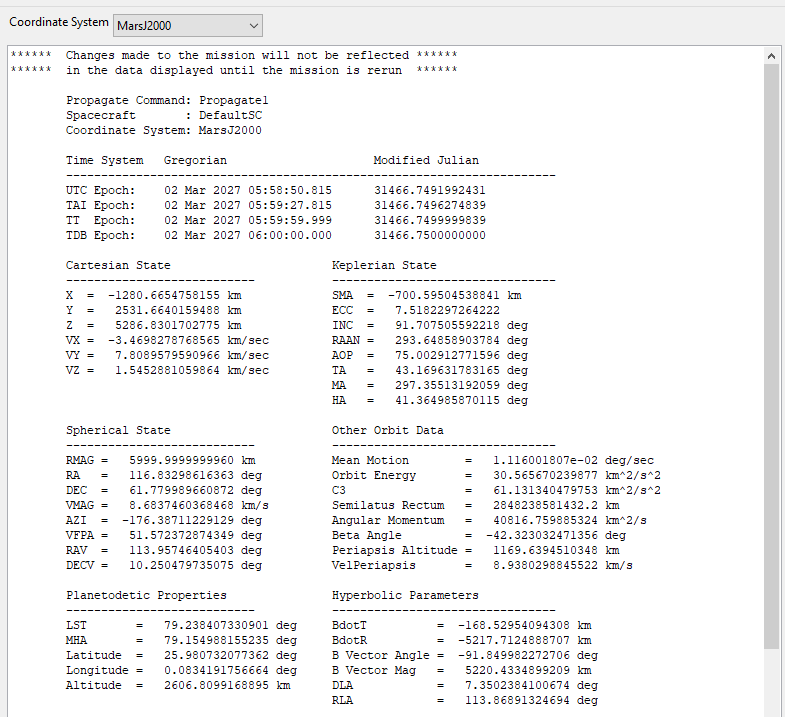
\includegraphics[width=0.95\linewidth]{Constraint_Scripting_mars_gmat_arrival.png}
	\caption{Mars Arrival State in \ac{GMAT}}
\end{figure}

%%%%%%%%%%%%%%%%%%%%%
\subsection{Adding a Maneuver Constraint}
\label{sec:adding_a_maneuver_constraint}
%%%%%%%%%%%%%%%%%%%%%

Let's add a maneuver constraint in our \verb|EVM_freepoint| mission. Create a new \verb|.emtgopt| file using either your \verb|EVM_freepoint.emtgopt| or \verb|EVM_freepoint_boundary_constraint.emtgopt| file and name it \verb|EVM_freepoint_maneuver_constraint.emtgopt|. Change the mission name to \newline``EVM\_freepoint\_maneuver\_constraint'' in the Global Options tab in PyEMTG. Open the ``Solver Options'' tab in PyEMTG and change the ``Inner-loop Solver Mode'' to ``Evaluate TrialX'' and select a previous \verb|.emtg| solution file from either the \verb|EVM_freepoint| or \verb|EVM_freepoint_boundary_constraint| results as the ``Trial decision vector''. Save the file in PyEMTG. Open both the \newline\verb|EVM_freepoint_maneuver_constraint.emtgopt| file and the \verb|.emtg| solution file you just used as a ``Trial decision vector'' in text editors.

\noindent Examine Journey 0 in the \verb|.emtg| file and find the date of the first \verb|chem burn| entry. We're going to apply a maneuver constraint which forces this \ac{DSM} to be on a different day. Convert the date of the \ac{DSM} to an \ac{MJD} epoch using one of the calendar tools in PyEMTG such as the one in the Global Options tab. For example 5 May 2026 would convert to 61165.0. In the Journey 0 section of your \verb|EVM_freepoint_maneuver_constraint.emtgopt| file change the \verb|BEGIN_MANEUVER_CONSTRAINT_BLOCK| by adding a constraint like the one below. This syntax indicates that the Phase 0 (\verb|p0|) burn 0 (\verb|b0|) absolute epoch \verb|epoch_abs| should fall between MJD 61160.0-61162.0. Change the epochs as appropriate so that the constraint is forcing the maneuver to occur in a window that \emph{does not} include the maneuver epoch in the \verb|.emtg| file. Save the \verb|.emtgopt| file. 

\begin{verbatim}
    BEGIN_MANEUVER_CONSTRAINT_BLOCK
    p0b0_epoch_abs_61160.0_61162.0
    END_MANEUVER_CONSTRAINT_BLOCK
\end{verbatim}

\noindent Run the file using either the command line or PyEMTG (if you use PyEMTG, ensure that you \emph{re-open} the \verb|.emtgopt| file as updates in your text editor do not sync to PyEMTG if the file is still open in PyEMTG). You should see terminal output similar to what is shown below indicating that the maneuver constraint is violated. Additionally, in the run folder created inside your results directory your \verb|.emtg| file should be named \verb|FAILURE_EVM_freepoint_maneuver_constraint.emtg| indicating that the solution was not feasible. Note that the somewhat confusing \verb|Decision vector is feasible| terminal output simply means that the trial decision vector is within it's upper and lower bounds \emph{not} that it meets all the constraints.


\begin{verbatim}
    Acquired infeasible point with feasibility 0.000460129
    Worst constraint is F[1]: j0p0MGAnDSMsForwardSubPhase0: maneuver epoch absolute 
    constraint with violation 0.000460129
    Decision vector is feasible.
    EMTG run complete.
    Press enter to close window.
\end{verbatim}

\noindent Now try changing the solver mode to ``Monotonic Basin Hopping'' in the Solver Options tab of PyEMTG or by changing the text file \verb|run_inner_loop| option to \verb|1| and running \ac{EMTG}. Open the resulting \verb|.emtg| file and verify that the first \ac{DSM} in Journey 0, Phase 0 occurs between the dates you set in the maneuver constraint block. For example, the chemical burn shown below on 5/2/2026 (\ac{JD} 2461162.50034601) converts to a \ac{MJD} of 61162.00034601 (\ac{MJD} = \ac{JD} - 2,400,000.5) which meets the constraint within \ac{EMTG}'s tolerance. 

\begin{verbatim}
    10 | 2461157.44477123 |   4/26/2026 |        coast | 
    11 | 2461162.50034601 |    5/2/2026 |    chem_burn |
    12 | 2461162.50034601 |    5/2/2026 |  match_point |
\end{verbatim}



\end{document}





















